\chapter{Fuel system production process} \label{Fuel system production process}
\markboth{\MakeUppercase{Fuel system production process}}{\MakeUppercase{Fuel system production process}}

The manufacturing of a complete fuel system is the result of multiple production stages: 

\begin{itemize}
    \item Material Supply: plastic material is stored in dedicated silos into the plant. The material supply equipment is directly connected to the extrusion blow-moulding machine in order to continuously feed the extruders with new raw material.
    \item Extrusion blow-moulding: it is the core manufacturing process of the entire production line. During this stage raw material is transformed in a hollow fuel tank. 
    \item Post Cooling: once the fuel tank has been blown, it enters a phase of post-mould cooling, where its temperature is lowered a second mould. This operation allows for the stabilisation of the tank dimensions.
    \item Finishing: during the finishing stage the hollow tank is cut in different areas and extra components are welded on it.
    \item Assembly: finally, some parts such as the filler pipe are assembled on the tank and every tank is checked to detect possible leaks.
\end{itemize}

The full process is outlined in Figure \ref{fig:Full_production_process}.

\begin{figure}
\centerline{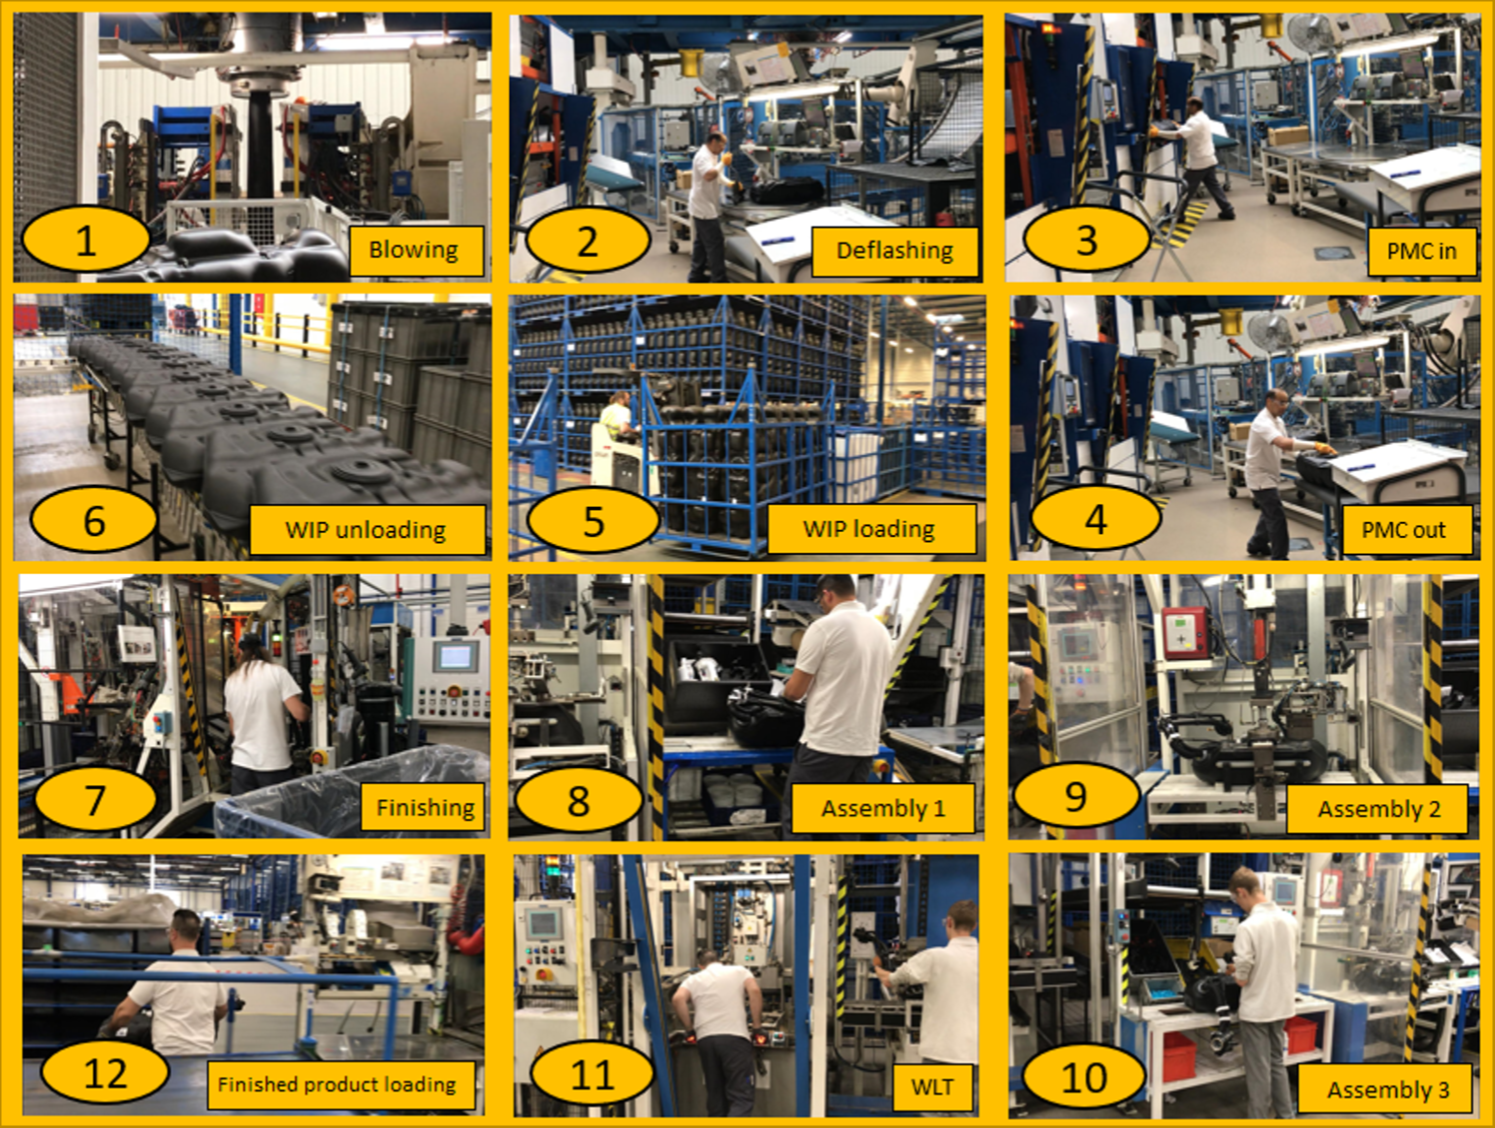
\includegraphics[scale=0.4]{images/appendix_B/Blow_molding_process.png}}
\caption{Full production process}
\label{fig:Full_production_process}
\end{figure}